%!TEX TS-program = xelatex

\documentclass[a4paper,12pt, landscape]{article}

\usepackage[english,russian]{babel}   %% загружает пакет многоязыковой вёрстки
\usepackage{fontspec}      %% подготавливает загрузку шрифтов Open Type, True Type и др.
\defaultfontfeatures{Ligatures={TeX},Renderer=Basic}  %% свойства шрифтов по умолчанию
\setmainfont[Ligatures={TeX,Historic},
SmallCapsFont={Brill},
SmallCapsFeatures={Letters=SmallCaps}]{Brill} %% задаёт основной шрифт документа
\setsansfont{Brill}                    %% задаёт шрифт без засечек
\setmonofont{Noto Sans Ethiopic}
\usepackage{indentfirst}

%%% Дополнительная работа с математикой
\usepackage{amsmath,amsfonts,amssymb,amsthm,mathtools} % AMS
\usepackage{icomma} % "Умная" запятая: $0,2$ --- число, $0, 2$ --- перечисление

%%% Работа с картинками
\usepackage{wrapfig} % Обтекание рисунков текстом
\usepackage{subcaption}
\usepackage{rotating}
\usepackage{fixltx2e}
\usepackage{hhline}
\usepackage{lscape}
\usepackage[usenames,dvipsnames,svgnames,table,rgb]{xcolor}%пакет для использования цветов 

\usepackage{enumitem}
\setlist{nolistsep, leftmargin=5mm}

%%% Работа с таблицами
\usepackage{array,tabularx,tabulary,booktabs} % Дополнительная работа с таблицами
\usepackage{longtable}  % Длинные таблицы
\usepackage{multirow} % Слияние строк в таблице

\usepackage{multicol} % Несколько колонок

%%% Страница
\usepackage{extsizes} % Возможность сделать 14-й шрифт
\usepackage[twocolumn]{geometry} % Простой способ задавать поля
	\geometry{top=12mm}
	\geometry{bottom=13mm}
	\geometry{left=13mm}
	\geometry{right=9mm}

%\usepackage{fancyhdr} % Колонтитулы
% 	\pagestyle{fancy}
 	%\renewcommand{\headrulewidth}{0pt}  % Толщина линейки, отчеркивающей верхний колонтитул
% 	\lfoot{Нижний левый}
% 	\rfoot{Нижний правый}
% 	\rhead{Верхний правый}
% 	\chead{Верхний в центре}
% 	\lhead{Верхний левый}
%	\cfoot{Нижний в центре} % По умолчанию здесь номер страницы

\usepackage{setspace} % Интерлиньяж
%\onehalfspacing % Интерлиньяж 1.5
%\doublespacing % Интерлиньяж 2
\singlespacing % Интерлиньяж 1

\usepackage{lastpage} % Узнать, сколько всего страниц в документе.
\usepackage{soul} % Модификаторы начертания
\usepackage{bbding}
\usepackage{hyperref}
\usepackage[usenames,dvipsnames,svgnames,table,rgb]{xcolor}
\hypersetup{				% Гиперссылки
    colorlinks=true,       	% false: ссылки в рамках; true: цветные ссылки
    linkcolor=black,          % внутренние ссылки
    citecolor=black,        % на библиографию
    filecolor=black,      % на файлы
    urlcolor=ForestGreen          % на URL
}

\usepackage{environ}
\makeatletter
\newsavebox{\measure@tikzpicture}
\NewEnviron{scaletikzpicturetowidth}[1]{%
	\def\tikz@width{#1}%
	\def\tikzscale{1}\begin{lrbox}{\measure@tikzpicture}%
		\BODY
	\end{lrbox}%
	\pgfmathparse{#1/\wd\measure@tikzpicture}%
	\edef\tikzscale{\pgfmathresult}%
	\BODY
}
\makeatother

\usepackage{pgfplots}
\usepackage{pgfplotstable}
\usepackage{verbatim}

\usepackage{attachfile2}
 \attachfilesetup{appearance=true,
color=0 0 0
 }

%%% Лингвистические пакеты
%\usepackage{savetrees} % пакет, который экономит место
\usepackage{forest} % для рисования деревьев
\usepackage{vowel} % для рисования трапеций гласных
\usepackage{natbib}
\bibpunct[: ]{[}{]}{;}{a}{}{,}
\usepackage[nogroupskip,nopostdot, nonumberlist]{glossaries}
%\usepackage{glossary-mcols} 
%\setglossarystyle{mcolindex}
\usepackage{philex} % пакет для примеров
\addto\captionsrussian{% Replace "english" with the language you use
\renewcommand{\refname}{}
\renewcommand{\glossaryname}{Список глосс}
}
\newcommand{\mytem}{\item[$\circ$]}

\usepackage{todonotes}
\newcounter{mycomment}
\newcommand{\mycom}[1]{
\refstepcounter{mycomment}%
{%
\setstretch{0.7}% spacing
\todo[color=blue!20!white, inline]{%
\textbf{ГМ\themycomment:}~{\footnotesize #1}}%
}}
\renewcommand{\thesection}{\arabic{section}.}
\renewcommand{\thesubsection}{\arabic{section}.\arabic{subsection}}
\setlength{\columnsep}{1.6cm}

\usepackage{sectsty}
\sectionfont{\normalsize}
\subsectionfont{\normalsize}
\usepackage{titlesec}
\titlespacing*{\section}
{0pt}{2ex plus 0ex minus .2ex}{0ex plus .2ex}
\titlespacing*{\subsection}
{0pt}{2ex plus 0ex minus .2ex}{0ex plus .2ex}
\newlength{\bibitemsep}\setlength{\bibitemsep}{.2\baselineskip plus .05\baselineskip minus .05\baselineskip}
\newlength{\bibparskip}\setlength{\bibparskip}{0pt}
\let\oldthebibliography\thebibliography
\renewcommand\thebibliography[1]{%
	\oldthebibliography{#1}%
	\setlength{\parskip}{\bibitemsep}%
	\setlength{\itemsep}{\bibparskip}%
}
\begin{document}
\begin{flushright}
	{\footnotesize Г. Мороз, а. Ходзь, Республика Адыгея}
\end{flushright}
\begin{center}{\Large Исследование скорости речи: кубанский диалект\footnote{Автор выражает благодарности:
\begin{itemize}
\mytem Ване Левину, Саше Мартыновой, Лене Пасальской и Соне Сиговой за помощь в придумывании историй;
\mytem Тане Руссите за рисунки;
\mytem информантам ... за неоценимую помощь в проведении исследования;
\mytem ... за комментарии.
\end{itemize}}}
\end{center}
{\noindent\footnotesize последняя версия: \textbf{\href{https://goo.gl/qMgtOd}{https://goo.gl/qMgtOd}}}
\vspace{5mm}
\tableofcontents
\vfill
{~}\\
\pagebreak
\section{Введение}
\noindent Судя по всему, о скорости речи говорили еще в начале XX века, но первые квантитативные исследования, начались, видимо, с работ \citep{goldman54} и \citep{goldman56}; и с самых ранних работ данная тема затрагивала еще и некоторые аспекты психиатрии.
\par В исследовании \citep{goldman54} исследовались по три интервью от пяти пациентов, собранных тремя психиатрами. В качестве характеристики скорости речи используется количество слов в минуту и стандартное отклонение полученной величины. В следующей работе \citep{goldman56} автор был более эксплицитен и ввел некоторые важные понятия:
\begin{itemize}
\mytem общая скорость речи (total or overall Speech Rate), которая высчитывается по формуле ${ns}/t$, где ${ns}$ --- это количество слогов во всех высказываниях, a $t$ --- общая длительность всех высказываний.
\mytem скорость артикуляции или абсолютная скорость речи (Articulation Rate), которая высчитывается по формуле $ns/ts$, где $ns$ --- это количество слогов во всех высказываниях, a $ts$ --- время чистого говорения.
\mytem пропорциональная длительность пауз, которая высчитывается по формуле $tp/t$, где $tp$ --- это длительность пауз во всех высказываниях, a $t$ --- общая длительность всех высказываний.
\mytem скорость дыхания (Respiration Rate), которая по формуле $ni/t$, где ${ni}$ --- это количество вдохов во всех высказываниях, a $t$ --- общая длительность всех высказываний.
\end{itemize}
\par Среди результатов работы \citep{goldman56} отмечается отрицательная корреляция между общей скоростью речи и пропорциональной длительностью пауз, т. е. чем длиннее и чем дольше паузы, тем меньше общая скорость речи. В исследовании также подчеркивается, что скорость дыхания, измеряемая в процессе речи, отличается от действительной скорости дыхания, так как в ней происходит выдыхательная задержка, вызванная процессом речепроизводства.
\par \citep{fonagy60}
\par \citep{osser64}
\par \citep{barik77}
\par \citep{vaane82}
\par \citep{brown85}
\par \citep{uhmann92}
\par \citep{zellner94}
\par \citep{roach98}
\par \citep{dellwo03}
\par \citep{pellegrino04} и \citep{pellegrino11}
\par \citep{hilton11}
\par \citep{pellegrino11}
\par \citep{stepanova11}
\par \citep{kendall13}
\par \citep{bosker15}
\par \citep{bosker16}
\section{Ход эксперимента}
\section{мысли}
\begin{itemize}
\mytem не только все усреднить --- скользящее среднее покажет изменении скорости по ходу рассказа
\mytem естественно считать слова странно, так как понятие "слова" далеко от универсального.
\end{itemize}
\pagebreak
\footnotesize
\bibliographystyle{chicago}
\bibliography{bibliography}
\normalsize
\section{Приложения}
\subsection{Приложение 1: изображения Тани Русситы}
\noindent 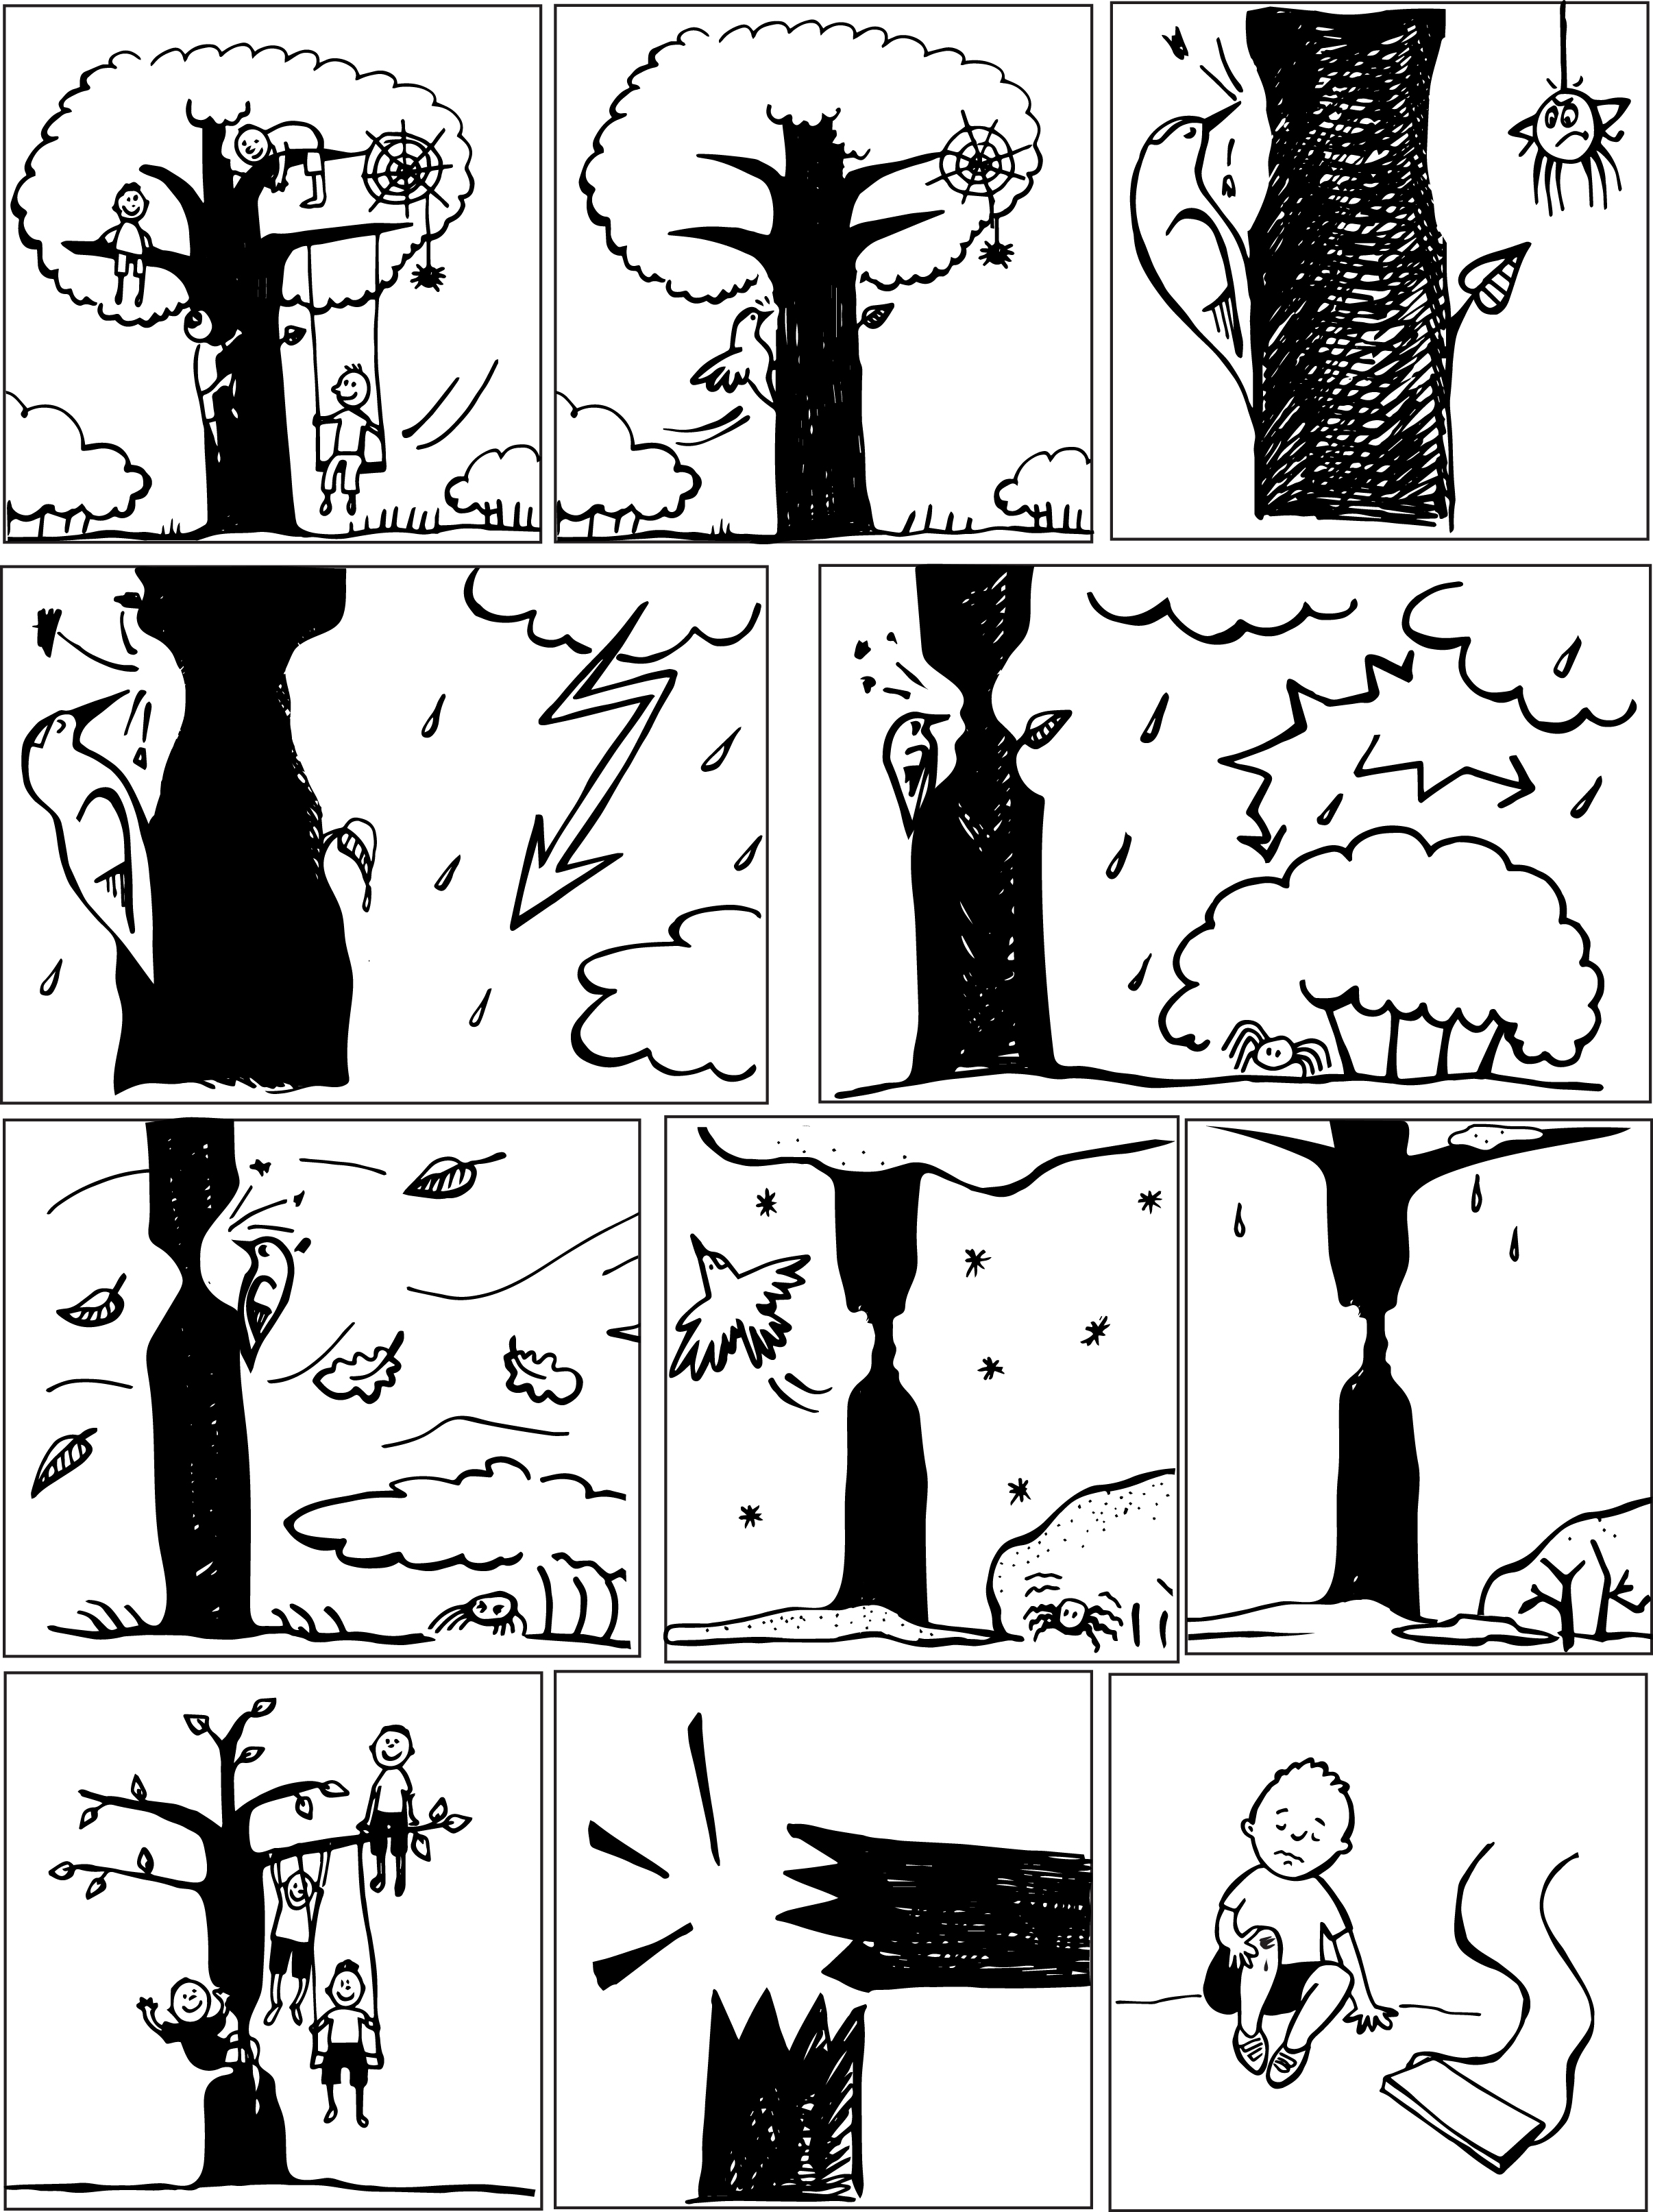
\includegraphics[width=\linewidth]{pauk.jpg}\\
\pagebreak\\
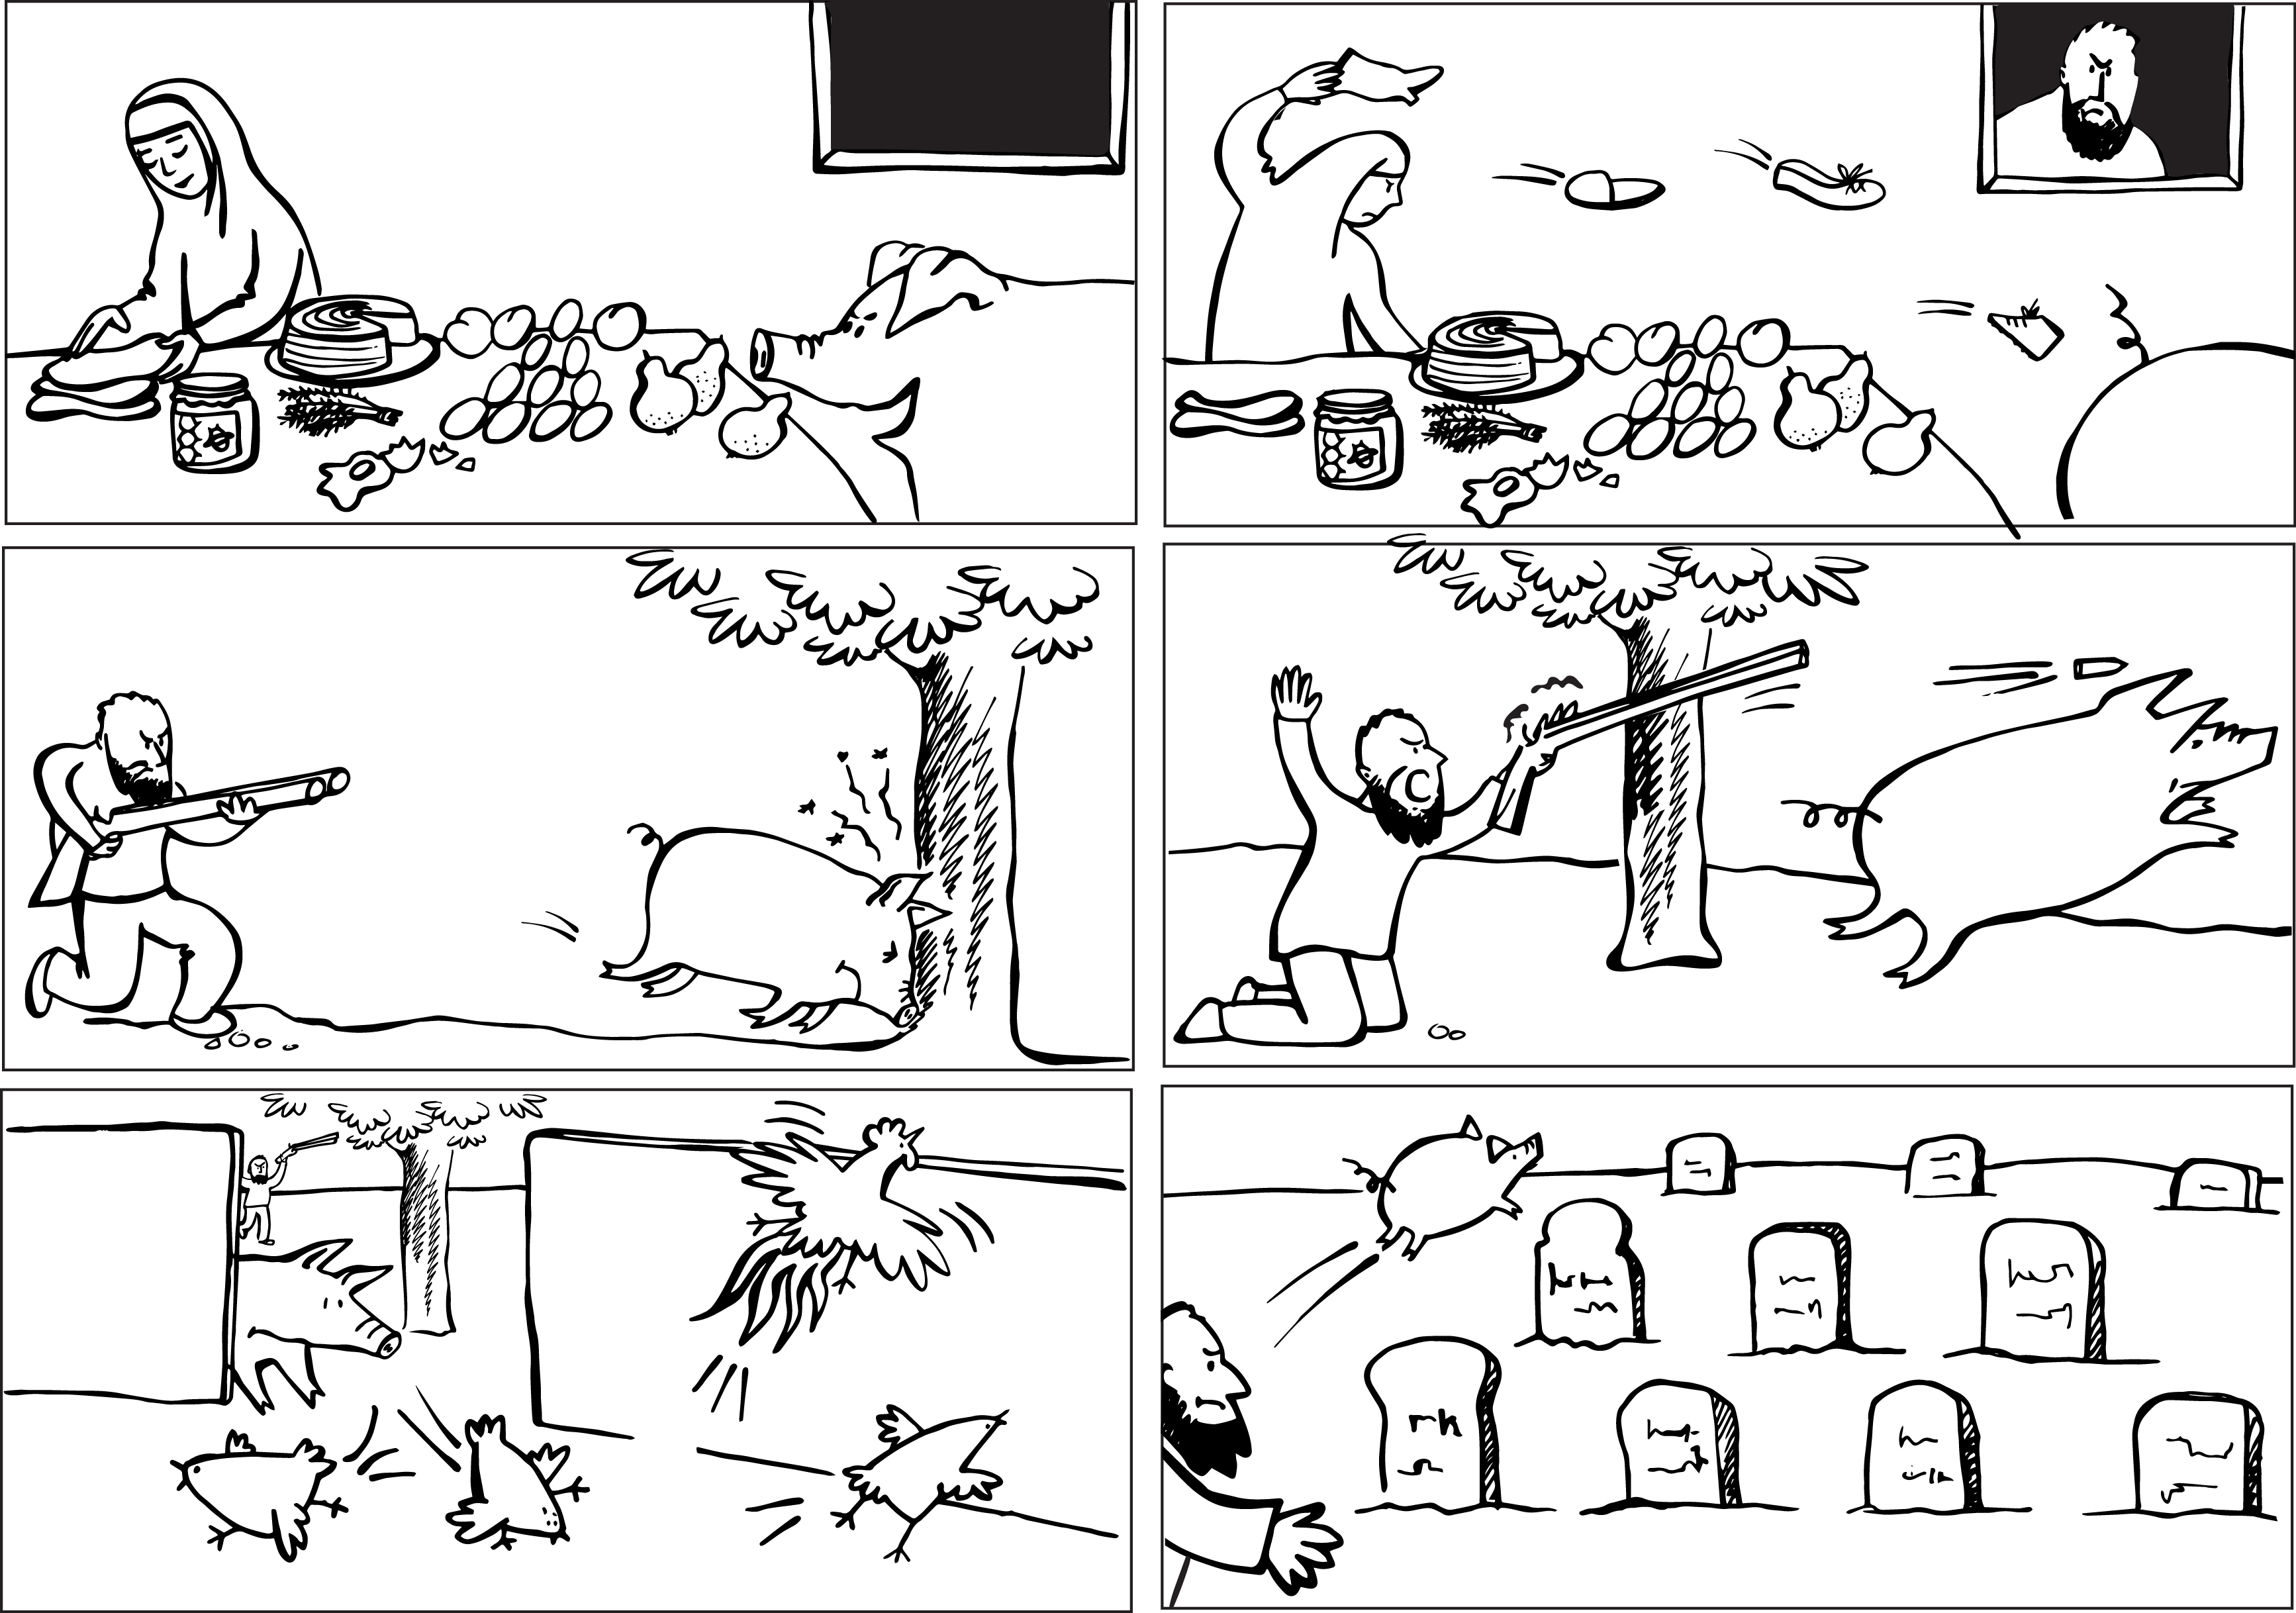
\includegraphics[width=\linewidth]{svinja.jpg}\\
\pagebreak
\subsection{Приложение 2: стихотворение Алима Кешокова}
{~}\medskip\\
\noindent Зыхэс удз Iувыр ирецIынэ,\\
И Iэщхьэр лъагэу дэхьеяуэ\\
Хъыджэбз нэкIуплъым епщ хупцIынэ,\\
Щхьэщысщ ар Iэнлъэм зигъэзхъауэ.\medskip\\
ЕIуящIэ защIэу щIалэ куэди\\
КъетIысэкIауэ мэгушыIэ.\\
И уз а пщафIэми укIуэди,\\
Сыт къыхуапсэлъми зешыIэ.\medskip\\
ТIэкIу зигъэщхъакъэ --- псори маплъэ,\\
А щIалэр зэплъыр къыпхуэмыщIэ,\\
Хъыджэбзырщ зыщIэр псом я пIалъэ ---\\
Зигу къэплъым и Iур ирегъущIэ.\medskip\\
И щхьэцыр пщащэм ирекъуэкIыр,\\
Хьэжыгъэр нэIум къытощащэ.\\
Гу лъумытэну я гум къэкIым,\\
ЩIалэжьхэр къеплъмэ мэIущащэ.\medskip\\
Я мэлхэр шытхым щхьэдэхами,\\
Мэлыхъуэр зыкIи мыгузавэ.\\
Дэтхэнэм жьэкIэ сыт жиIами,\\
Я плырыр псалъэм щIрагъавэ.\medskip\\
Зырыз мэл хъущэу къыдахуащ,\\
АрщхьэкIэ псоми зыщ ягъэхъур.\\
А хъыджэбз пщафIэм дихьэхащ --- \\
Апхуэдэу махуэр жэщ ягъэхъур. \medskip\\
Сыт щIалэ жанхэри зезыхьэр?\\
Мэлыхъуэм я гур хьэхугъуафIэщ,\\
Хъыджыбзым ищIрэ щIакхъуэ Iыхьэ,\\
Iухуакъэ, ишхыр хъунущ мафIэ.\medskip\\
\textit{Алим КIыщокъуэ, Тхыгъэхэр, томихым щызэхуэхьэсауэ ---  Налщык: <<Эльбрус>>, 2004. --- н. 147}
\pagebreak
\subsection{Приложение 3: код в PRAAT}
\subsection{Приложение 4: код в R}
\end{document}